%======================= DOCUMENTO ==================================================
Il manipolatore IRB 120 per poter essere gestito e per poter funzionare necessita di ricevere dall'esterno sia dei segnali di controllo che di alimentazione: di questo compito se ne occupa il controller IRC 5 Compact \emph{(Industrial Robot Controller)} (figura~\vref{fig:IRC5}), un'unità di controllo compatta che ha in sé tutti i benefici del IRC5, tra cui la precisione dell’analisi del movimento e l’utilizzo del
linguaggio di programmazione \textsc{rapid}, oltre a dimensioni nettamente ridotte.
\begin{figure}
	\centering
	\includegraphics[width=0.45\textwidth]{Immagini/IRC5}
	\caption{IRC5 Compact controller}
	\label{fig:IRC5}
\end{figure}

La parte di controllo della movimentazione, è individuata dalla presenza di un anello in retroazione sul sistema, in grado di valutare l'uscita e di andare a confrontarla con il valore di riferimento posto in ingresso. Questo feedback della traiettoria e della movimentazione non deve però essere esplicitamente sviluppato come un blocco a se stante, ma risulta già essere sviluppato all'interno del controllore stesso.
IRC5 Compact consente infatti ai robot di eseguire le proprie attività ad altissima efficienza, grazie ad una modellazione dinamica avanzata, permettendo di ottimizzare automaticamente le prestazioni riducendo i tempi di ciclo ($QuickMove^{TM}$) e garantendo che il percorso seguito dal robot sia lo stesso di quello programmato, indipendentemente dalla velocità di movimento ($TrueMove^{TM}$).

La tecnologia di IRC5 di ABB consente di prevedere il movimento del robot, garantendo prestazioni elevate, senza necessità di messa a punto da parte del programmatore, ovvero senza la necessità di dover andare a gestire il controllo sulla posizione.

\emph{Tu programmi, e lui esegue alla perfezione}.

Nella nostra applicazione, come in tutte le applicazioni che vanno a fare uso dei manipolatori industriali ABB, la presenza dell'IRC5 è inoltre fondamentale perchè permette di offrire una via per interfacciarsi e per gestire la movimentazione del braccio: questo è possibile grazie al fatto che esso supporta tutti i bus di campo attualmente in commercio in maniera tale che il robot possa integrarsi in ogni tipo di rete. 



Tra le numerose funzioni di networking ricordiamo il socket messaging (scambio di messaggi TCP/IP) e la possibilità di interfacciarsi con diversi sensori e accessi remoti: questo argomento è approfondito nella sottosezione~\vref{subsec:InterfaceIRC5}.

A livello "pratico", il controllore presenta delle interfacce destinate a gestire la parte di alimentazione e/o la parte di controllo del movimento del manipolatore: andiamo ora ad analizzare velocemente quelli che sono i principali collegamenti che il controllore offre.
\section{Pannello di controllo}
Il controller IRC5 presenta a bordo, oltre ad una serie di collegamenti, che gli permette di interfacciarsi al mondo esterno, anche una serie di pulsanti/interruttori situati sul pannello anteriore dell’IRC5 Compact.

\subsection{Pulsanti e interruttori}
La figura~\vref{fig:FrontPanelIRC5_1} mostra i pulsanti e gli interruttori situati sul pannello anteriore del controller IRC5 Compact.
\begin{figure}[h]
	\centering
	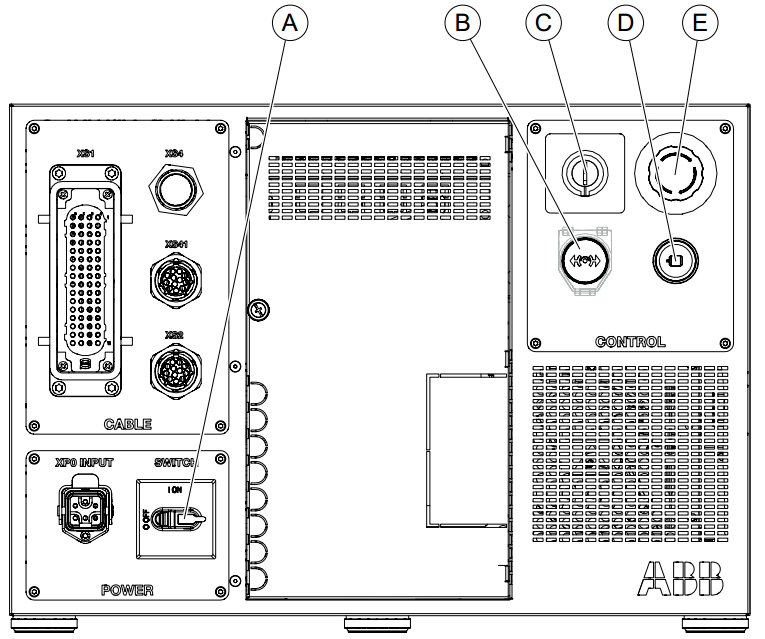
\includegraphics[width=0.5\textwidth]{Immagini/Pulsanti_Interruttori_IRC5}
	\caption{Pulsanti e interruttori presenti sul pannello anteriore del controller IRC5}
	\label{fig:FrontPanelIRC5_1}
\end{figure}
Le loro funzioni sono:
\begin{description}
	\item[A:] Interruttore principale di alimentazione
	\item[B:] Pulsante di rilascio dei freni che permette di modificare manualmente la posizione degli assi del manipolatore.
	\item[C:] Interruttore di scelta modalità di funzionamento del sistema robotico, la quale può essere: 
	\begin{itemize}
		\item \emph{Automatica}: definibile come “modalità di produzione” in cui il manipolatore si muove secondo quelle che sono le istruzioni RAPID (capitolo~\vref{text:RAPID}) che sono caricate a bordo del controllore. In questa modalità di funzionamento la velocità non risulta essere limitata, ma bensì dipende da quelle che sono le informazioni di velocità inserite all’interno della codifica delle istruzioni di movimento.
		\item \emph{Manuale}: in questa modalità il controllo avviene manualmente tramite il jog sulla flex pendant (figura ~\vref{text:FlexPendant}); la velocità di movimento risulta invece essere limitata a 250 mm/s.
	\end{itemize}
	\item[D:] Motori inseriti
	\item[E:] Arresto di emergenza: la pressione di questo tasto si rende necessaria nel momento in cui si attiva la modalità di funzionamento automatica. In particolar modo essa permette di attivare i motori che inizialmente risultano essere in blocco per motivi di sicurezza.
\end{description}
\subsection{Interfacce di collegamento}
\label{subsec:InterfaceIRC5}
Si analizzeranno, in prima battuta, le interfacce che permettono al controllore IRC5 di collegarsi al manipolatore IRB 120, fornendogli tutti i segnali necessari. In seconda battuta andremo ad  rapidamente i collegamenti che il controllore stesso presenta verso il "mondo esterno".
\newpage
Partiamo analizzando i collegamenti interni tra manipolatore e controller in figura~\vref{fig:FrontPanelIRC5_2}:
\begin{figure}[h]
	\centering
	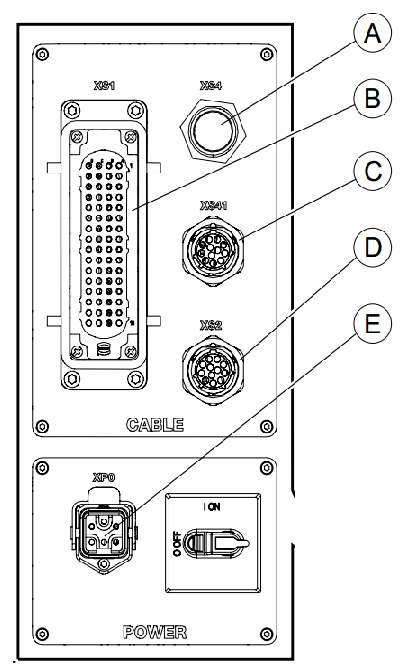
\includegraphics[width=0.3\textwidth]{Immagini/Connettori_IRC5}
	\caption{Connettori presenti sul pannello anteriore del controller IRC5}
	\label{fig:FrontPanelIRC5_2}
\end{figure}
\begin{description}
	\item[A:] Connessione alla FlexPendant
	\item[B:] Collegamento dell'alimentazione al robot
	\item[C:] Collegamento degli assi aggiuntivi
	\item[D:] Collegamento del robot
	\item[E:] Collegamento dell'alimentazione di rete
\end{description}
Il pannello di controllo dell’IRC5, oltre ai collegamenti esposti in precedenza, presenta altre porte di comunicazione, che permettono al controller di entrare in relazione con un PC/Sistema esterno.

In quello che è definito come il gruppo "computer" troviamo diversi collegamenti come si vede in figura~\vref{fig:ComputerGroup_IRC5}.
\begin{figure}
	\centering
	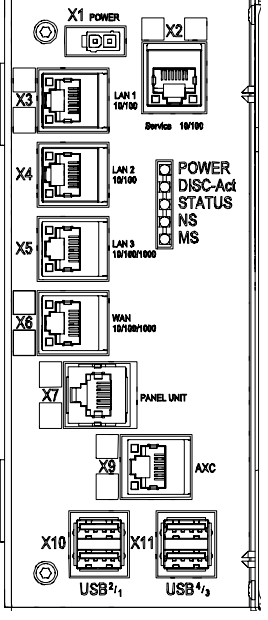
\includegraphics[width=0.30\textwidth]{Immagini/ConnettoriSulComputer}
	\caption{Porte di comunicazione IRC5}
	\label{fig:ComputerGroup_IRC5}
\end{figure}
I due collegamenti principali sono:
\begin{description}
	\item[Porta di servizio \textsl{X2}:]\label{item:Porta_servizio} questa porta è destinata ai tecnici di servizio e ai programmatori che si collegano direttamente al controller con un PC.
	La porta di servizio è configurata con un indirizzo IP fisso, che è identico per tutti i controller e non può essere modificato, ed è dotata di un server DHCP che assegna automaticamente un indirizzo IP al PC collegato: quindi, nel momento in cui si va a gestire la movimentazione del manipolatore tramite RobotStudio (capitolo~\vref{text:RAPID}), il PC deve essere connesso al controller tramite questa porta.
	Durante il collegamento il PC deve essere impostato su “Ottieni automaticamente un indirizzo IP” come descritto in Service PC information nel Boot Application della Flex Pendant (capitolo~\vref{chapter:FlexPendant}).
	
	\item[Porta di rete della fabbrica \textsl{X6}:] la porta di rete di fabbrica (WAN) è una porta pubblica destinata al collegamento del controller a una rete interna: per completezza si riporta in figura~\vref{fig:ComputerGroup_IRC5} una panoramica dei collegamenti possibili via Ethernet/USB. 
	Le impostazioni di rete possono essere configurate con qualsiasi indirizzo IP fornito, in genere, dall'amministratore della rete: per il PC dipendono dalla configurazione della rete medesima da parte dell’amministratore di rete.
	Questo ci permette di affermare che, un secondo modo per comunicare con il controllore, può essere tramite una rete (cablata o meno) alla quale risulta essere connesso il controllore stesso.
	Per la porta WAN non si possono utilizzare i seguenti indirizzi IP, in quanto già assegnati ad altre funzioni sul controller IRC5:
	\begin{itemize}
		\item 192.168.125.0 - 255
		\item 192.168.126.0 - 255
		\item 192.168.127.0 - 255
		\item 192.168.128.0 - 255
		\item 192.168.129.0 - 255
		\item 192.168.130.0 - 255
	\end{itemize}
	La porta WAN non può trovarsi su una subnet con uno degli indirizzi IP riservati sopra riportati. Se occorre utilizzare una subnet mask nell'intervallo B della classe di indirizzi, specificare un indirizzo privato di classe B per evitare conflitti.
\end{description}
\subsection{Morsettiera di suppporto}
Sul pannello di controllo dell'IRC5 Compact è inoltre presente una morsettiera che permette di effettuare collegamenti esterni (a livello \emph{"elettrico"}). Vediamo quelli che sono i principali collegamenti e le loro funzionalità.
\begin{description}
	\item[XS7-XS8-XS9] Questi connettori sono collegati internamente alla scheda di sicurezza e contengono i seguenti segnali:
	\begin{itemize}
		\item Arresto automatico
		\item Arresto generale
		\item Arresto di emergenza esterno
		\item Alimentazione esterna
	\end{itemize}
	\item[XS12\dots XS15] Questi connettori sono collegati internamente all'unità I/O: essi contengono 16 segnali di ingresso digitali, 16 segnali di uscita digitali,
	24 V e 0 V per le uscite e 0 V per gli ingressi. 24 V e 0 V devono essere di	alimentazione esterna.
	\item[XS16] Questo connettore è collegato internamente all'unità I/O e all'unità di
	distribuzione dell'alimentazione a 24 V con un assorbimento di corrente non superiore a 6A.
\end{description}
%====================================================================================